%File: formatting-instructions-latex-2024.tex
%release 2024.0
\documentclass[letterpaper]{article} % DO NOT CHANGE THIS
\usepackage{aaai24}  % DO NOT CHANGE THIS
\usepackage{times}  % DO NOT CHANGE THIS
\usepackage{helvet}  % DO NOT CHANGE THIS
\usepackage{courier}  % DO NOT CHANGE THIS
\usepackage[hyphens]{url}  % DO NOT CHANGE THIS
\usepackage{graphicx} % DO NOT CHANGE THIS
\urlstyle{rm} % DO NOT CHANGE THIS
\def\UrlFont{\rm}  % DO NOT CHANGE THIS
\usepackage{natbib}  % DO NOT CHANGE THIS AND DO NOT ADD ANY OPTIONS TO IT
\usepackage{caption} % DO NOT CHANGE THIS AND DO NOT ADD ANY OPTIONS TO IT
\frenchspacing  % DO NOT CHANGE THIS
\setlength{\pdfpagewidth}{8.5in}  % DO NOT CHANGE THIS
\setlength{\pdfpageheight}{11in}  % DO NOT CHANGE THIS
%
% These are recommended to typeset algorithms but not required. See the subsubsection on algorithms. Remove them if you don't have algorithms in your paper.
\usepackage{algorithm}
\usepackage{algorithmic}

%
% These are are recommended to typeset listings but not required. See the subsubsection on listing. Remove this block if you don't have listings in your paper.
\usepackage{newfloat}
\usepackage{listings}
\DeclareCaptionStyle{ruled}{labelfont=normalfont,labelsep=colon,strut=off} % DO NOT CHANGE THIS
\lstset{%
	basicstyle={\footnotesize\ttfamily},% footnotesize acceptable for monospace
	numbers=left,numberstyle=\footnotesize,xleftmargin=2em,% show line numbers, remove this entire line if you don't want the numbers.
	aboveskip=0pt,belowskip=0pt,%
	showstringspaces=false,tabsize=2,breaklines=true}
\floatstyle{ruled}
\newfloat{listing}{tb}{lst}{}
\floatname{listing}{Listing}
%
% Keep the \pdfinfo as shown here. There's no need
% for you to add the /Title and /Author tags.
\pdfinfo{
/TemplateVersion (2024.1)
}

% DISALLOWED PACKAGES
% \usepackage{authblk} -- This package is specifically forbidden
% \usepackage{balance} -- This package is specifically forbidden
% \usepackage{color (if used in text)
% \usepackage{CJK} -- This package is specifically forbidden
% \usepackage{float} -- This package is specifically forbidden
% \usepackage{flushend} -- This package is specifically forbidden
% \usepackage{fontenc} -- This package is specifically forbidden
% \usepackage{fullpage} -- This package is specifically forbidden
% \usepackage{geometry} -- This package is specifically forbidden
% \usepackage{grffile} -- This package is specifically forbidden
% \usepackage{hyperref} -- This package is specifically forbidden
% \usepackage{navigator} -- This package is specifically forbidden
% (or any other package that embeds links such as navigator or hyperref)
% \indentfirst} -- This package is specifically forbidden
% \layout} -- This package is specifically forbidden
% \multicol} -- This package is specifically forbidden
% \nameref} -- This package is specifically forbidden
% \usepackage{savetrees} -- This package is specifically forbidden
% \usepackage{setspace} -- This package is specifically forbidden
% \usepackage{stfloats} -- This package is specifically forbidden
% \usepackage{tabu} -- This package is specifically forbidden
% \usepackage{titlesec} -- This package is specifically forbidden
% \usepackage{tocbibind} -- This package is specifically forbidden
% \usepackage{ulem} -- This package is specifically forbidden
% \usepackage{wrapfig} -- This package is specifically forbidden
% DISALLOWED COMMANDS
% \nocopyright -- Your paper will not be published if you use this command
% \addtolength -- This command may not be used
% \balance -- This command may not be used
% \baselinestretch -- Your paper will not be published if you use this command
% \clearpage -- No page breaks of any kind may be used for the final version of your paper
% \columnsep -- This command may not be used
% \newpage -- No page breaks of any kind may be used for the final version of your paper
% \pagebreak -- No page breaks of any kind may be used for the final version of your paperr
% \pagestyle -- This command may not be used
% \tiny -- This is not an acceptable font size.
% \vspace{- -- No negative value may be used in proximity of a caption, figure, table, section, subsection, subsubsection, or reference
% \vskip{- -- No negative value may be used to alter spacing above or below a caption, figure, table, section, subsection, subsubsection, or reference

\setcounter{secnumdepth}{0} %May be changed to 1 or 2 if section numbers are desired.

% The file aaai24.sty is the style file for AAAI Press
% proceedings, working notes, and technical reports.
%

% Title

% Your title must be in mixed case, not sentence case.
% That means all verbs (including short verbs like be, is, using,and go),
% nouns, adverbs, adjectives should be capitalized, including both words in hyphenated terms, while
% articles, conjunctions, and prepositions are lower case unless they
% directly follow a colon or long dash
\title{COMP 370 Final Project -- Movie Release }
\author{
    %Authors
    % All authors must be in the same font size and format.
    Written by \\ Renee Li (261085984), Grace Liang (260884150), Daniel Liao (261099147)
}
\affiliations{
    %Afiliations
    McGill School Of Computer Science\\
    % If you have multiple authors and multiple affiliations
    % use superscripts in text and roman font to identify them.
    % For example,

    % Sunil Issar\textsuperscript{\rm 2}, 
    % J. Scott Penberthy\textsuperscript{\rm 3}, 
    % George Ferguson\textsuperscript{\rm 4},
    % Hans Guesgen\textsuperscript{\rm 5}
    % Note that the comma should be placed after the superscript

    3480 Rue University, Montreal, QC H3A 2A7\\
    % email address must be in roman text type, not monospace or sans serif
    renee.li@mail.mcgill.ca, grace.liang@mail.mcgill.ca, daniel.liao@mail.mcgill.ca
%
% See more examples next
}

%Example, Single Author, ->> remove \iffalse,\fi and place them surrounding AAAI title to use it
\iffalse
\title{My Publication Title --- Single Author}
\author {
    Author Name
}
\affiliations{
    Affiliation\\
    Affiliation Line 2\\
    name@example.com
}
\fi

\iffalse
%Example, Multiple Authors, ->> remove \iffalse,\fi and place them surrounding AAAI title to use it
\title{My Publication Title --- Multiple Authors}
\author {
    % Authors
    First Author Name\textsuperscript{\rm 1,\rm 2},
    Second Author Name\textsuperscript{\rm 2},
    Third Author Name\textsuperscript{\rm 1}
}
\affiliations {
    % Affiliations
    \textsuperscript{\rm 1}Affiliation 1\\
    \textsuperscript{\rm 2}Affiliation 2\\
    firstAuthor@affiliation1.com, secondAuthor@affilation2.com, thirdAuthor@affiliation1.com
}
\fi

\begin{document}

\maketitle

\begin{abstract}
This report examines the press coverage of \textit{Anora}, directed by Sean Baker, compared to two other films released on the same day, \textit{Conclave} and \textit{Venom 3}. We analyzed over 500 articles collected via NewsAPI and categorized the coverage into themes such as reviews, production, and performance to assess visibility and reception. Results indicate that \textit{Anora} received significantly less coverage than both \textit{Conclave} and \textit{Venom 3}, attributed to its independent film status, controversial subject matter, and smaller budget. However, \textit{Anora} garnered more reviews from independent critics, often focusing on social commentary, highlighting its critical prestige despite lower overall visibility. Our findings underscore the role of budget, subject matter, and distribution scale in shaping media coverage of films.
\end{abstract}

\section{Introduction}

From the award-winning director of The Florida Project, Sean Baker’s most recent film Anora continues with his interest in the American underclass and follows the tale of a stripper from Brooklyn who embarks on a whirlwind marriage to the immature son of a Russian oligarch. Our report seeks to examine the nature of the press surrounding Anora relative to two movies that came out the same day, Conclave and Venom 3. Besides sharing the same release day, Conclave was selected to see how Anora’s press compared to a fellow independent film while Venom 3 was chosen to examine how it compared to a franchise.  
After collecting, annotating, and analyzing a dataset of over 500 articles, we compiled our key findings. Of the articles found that were directly related to the movie Anora, the most common category of coverage was reviews which tended to evaluate aspects such as storytelling, artistry, and acting quality. The second most common aspect of coverage was film performance, specifically the awards it had been nominated for. Quantitatively, Anora received less overall coverage relative to Conclave and Venom 3. We attributed these findings to factors related to Anora being an independent film with a lower budget, inappropriate subject matter, and greater focus on artistry. 


\section{Data}
Across the three movies, Anora, Conclave, and Venom 3, we collected a total of 600 articles: 200 articles per movie title search query, or 100 articles per movie per week for the two weeks following the movie’s official release date. However, querying the second week of Anora’s release only yielded 60 results and after excluding articles that had been collected by the API but listed as “[removed],” the dataset consisted of 550 articles. For each article in our dataset, we gathered information on the article source, author, title, description, URL link, content, publication date, publisher, and category of focus. The focus field was self-defined and hand-coded but all the other fields were specified within the NewsAPI call. To ensure all posts were in English, we specified language = ‘en’ under the get\_everything() command. To ensure all posts had a very high likelihood of being related to one of the movies, we conducted separate queries for each movie, using the movie title (“Anora,” “Conclave,” and “Venom”) as the search keyword. 

Our other data collection parameters were determined by the fact that the NewsAPI free tier only allows you to pull articles from the past month with a maximum of 100 requests at once. Using the NewsAPI “everything” and “sortBy=relevancy” query, this meant we were limited to collecting only the top 100 results of a set time range. Thus, while there might be over 100 articles relevant to our topic in a certain time range, we would never be able to see beyond the first 100. As a result, we pulled 100 articles per week per movie title for the two consecutive weeks following the movie’s release in theaters in order to be as comprehensive as possible. By collecting data by the week instead of a larger time range, we hoped to reduce the amount of relevant articles that might have been excluded due to the upper limit of 100 articles. We also wanted to see that there existed irrelevant articles towards the bottom of our API call as an indication that all relevant articles were gathered. All three movies selected were released on the same day, October 25, 2024, to help simplify the date inputs and better standardize comparison. 

At first we attempted to collect data on the first and fourth weeks following the movie’s release date to see if that changed the nature of articles but found that the fourth week returned articles that were mostly irrelevant or unrelated. In our initial data collection attempts, we also specified the query results be sorted by publication date (sortBy=“publishedAt”) thinking it would remove an element of bias that we presumed the “relevancy” sort involved before realizing this did not change the collection of articles that were returned


\section{Methods}
Since Anora was chosen as our primary focus, we decided to analyze Conclave and Venom 3 as they have the same release date as Anora, and would provide the best reference point for comparing visibility and reception. We decided on collecting 2 weeks worth of articles for all three movies, with the goal of obtaining 100 of the most relevant articles from each week. The weeks for which we collected articles are October 25 to October 31 and November 1 to November 7. Choosing movies with the same release date and obtaining data from identical windows of time allowed us to have data that are as unbiased and comparable as possible, ensuring no particular movie was favored. We wrote a script in Python to obtain articles from NewsAPI.org and set the parameters as the name of the movie and the week that we are interested in. We used these parameters consistently for all our searches.

In order to evaluate what aspects of Anora news articles focused on, we created a typology for the foci of articles through two rounds of open coding. To get started, we modified our JSON dataset to be fitted for our open coding by using a script to add a “category” field to each movie article entry in all data sets. The first round of coding involved each group member independently annotating the first two weeks worth of articles on the movies Anora, Conclave, and Venom 3 respectively. The second round involved compiling the categories of the first round into seven distinct categories of article focus, and annotating our data again using the finalized set of categories. 

When coming up with categories for the articles, we intentionally included a “Duplicate” category since some of our articles mentioned two or more of the movies and an “Other films” category to account for articles that only mention other relevant films. These categories help account for the noise in our data. We also included a category for articles that were not about any movies in question at all so it could be excluded from the final dataset and calculated totals. To evaluate the amount of coverage Anora received relative to other movies that came out at a similar time, we calculated the frequency of each category of focus. We also calculated the amount of articles that were actually written about each movie by excluding articles that were not about the movie in question at all from the total amount of articles pulled. 

We created a TF-IDF algorithm based on the one outlined in Homework 11 to determine the ten words used most frequently for each category of focus and removed punctuation, numbers, and English stop words using the Natural Language Toolkit library. Using the scikit-learn TfIdfVectorizer made this easy, and we implemented a regex token pattern to ensure that we only matched word characters. We performed the TF-IDF calculations in two different ways: including and excluding the movie names from the final top ten. We chose this approach in an effort to better understand the impact of the movie names on the categories.


\section{Results}
In our first round of annotation, each member separately evaluated one of the three movies in order to identify themes general to any movie article and eliminate any categories that were overly specific. We came up with the following categories:

\textbf{Anora:} best films at the moment, director, societal impact, film review, awards and nominations, movie cast

\textbf{Conclave:} announcement, review, crew, cast, commercial performance, articles about movies that are not the one in question, articles not about movies at all

\textbf{Venom:} character relationships, narrative closure, post-credit speculations, box office performance, critical reception and humor, easter eggs and references, soundtrack and production, and speculative theories

Some categories were identified as specific to the nature of the movie. For example, Venom is part of the Marvel franchise so it had elements like post-credit scenes and cross-franchise references that Anora and Conclave did not have. After some discussion, we condensed our categories into seven final categories.



\subsection{Final Typology Definitions}
\textbf{Review:} Articles whose main focus is analyzing or evaluating a movie, discussing its artistic value or overall impact. Written by critics, they provide opinions for the quality and content of the film. 

\begin{itemize}
\item \textbf{Positive example:} The article title is “Anora and the changing depiction of sex work in Hollywood”. This article directly discusses the societal impact of the film, therefore is a positive example.

\item\textbf{Negative example:} The article title is “Sean Baker Talks ‘Anora’, Shooting On 35 mm and Winning the Palme d’Or”. This article is not included, because it focuses on the director’s experience as well as the production, and does not analyze the film itself.

\item\textbf{Edge case:} The article title is "Anora: Sean Baker's 'startlingly wise and tender' film is his most vivid creation yet'". Though the article heading mentions the director, the article is more of a review of the movie as opposed to commentary on the director.
\end{itemize}
\textbf{Production:} Articles whose main focus is the production process of the film, including aspects such as direction, cinematography, filming techniques, set design, costumes and other behind-the-scenes elements.
\begin{itemize}
\item\textbf{Positive example:} The article title is “Sean Baker Talks ‘Anora’, Shooting On 35 mm and Winning the Palme d’Or”. This article directly pertains to Production, because it talks about the director’s filming techniques such as shooting on a 35 mm film.
\item\textbf{Negative example:} The article title is "Weekend Box Office: 'Venom 3' Stays on Top". This article discusses the performance of Venom, but does not discuss anything regarding the production process of the film.
\item\textbf{Edge case:} "Anora director Sean Baker: What Mikey Madison did was so impressive. She shadowed lap dancers. She spent time in the club”. The title of the article is about the director commenting on one of the cast members, but it is more relevant to the effort put into the film by the cast, rather than the production of the film.
\end{itemize}
\textbf{Cast:} Articles whose main focus is commentary from or regarding the movie’s actors and actresses, including their performances, personal lives, casting experiences and interviews. 
\begin{itemize}
\item\textbf{Positive example:} The article title is “How Ivy Wolk Went From Shitposting to the Silver Screen”. This article talks about how Ivy Wolk was cast in Anora and therefore directly discusses the experience of the actress casting. 
\item\textbf{Negative example:} The article title is "Conclave Author Robert Harris on the Origin of His Best-Selling Vatican Thriller and Its Stunning Twist". This article is excluded because it discusses the author who wrote Conclave, but does not discuss the cast of the film. 
\item\textbf{Edge case:} “Sean Baker and Mikey Madison on the Scream star's new movie with a near-perfect Rotten Tomatoes score”. This article could fall under cast or performance based on the headline alone, but we categorized it as cast because the article is about the actress’s performance and experience in Anora and in another work, putting more emphasis on the actress than the performance of the film. 
\end{itemize}
\textbf{Performance:} Articles whose main focus is on the box office performance, viewership, awards, nominations and impact on the film industry.
\begin{itemize}
\item\textbf{Positive example:} The article title is “‘Anora’ Is the Hero Gothams Need”. This article falls under the category of performance, because it discusses the nominations that Anora has received which highlights the film’s performance.
\item\textbf{Negative example:} The article title is “Venom 3's Knull Actor Has Been Revealed \& It's A Marvel Veteran". This article is about the cast of the film since it is revealing the actor, and is therefore excluded from the category.
\item\textbf{Edge case:} “Gotham Awards Nominations Give ‘Anora,’ ‘Babygirl,’ ‘Nickel Boys’ a Boost”. This article talks about the performance of Anora as it discusses its nominations, however it also mentions other films and could be placed under that category. We have decided to place this article under the performance category, as it directly speaks about the performance of Anora. 
\end{itemize}
\textbf{Other films:} Articles whose main focus is related to movies but not the movie in question. 
\begin{itemize}
\item\textbf{Positive example:} The article title is “The Best New Movies of October 2024”. This article discusses all the current best movies in theatres, and therefore is not especially focused on any of the films we are interested in. We therefore included it in our category.
\item\textbf{Negative example:} The article title is “"ANORA Star Mikey Madison in Gucci at the 2024 LACMA Art+Film Gala". The article discusses the outfit that the main actress from Anora wears at a Gala, and is completely unrelated to other films. We therefore excluded it from this category.
\item\textbf{Edge case:} “‘Venom: The Last Dance’ Falls Short, but Look at ‘Conclave’ and ‘Anora’ Soar”. This article talks about other films, but also highlights the performance of Anora. We decided to include it under “Other films”, because the article description does not seem to put much focus on Anora itself. 
\end{itemize}
\textbf{Unrelated articles: }Articles whose main focus is not related to movies at all. We included this category to understand how many relevant vs irrelevant articles existed. 
\begin{itemize}
\item\textbf{Positive example:} The article name is “It’s the Most Hated Font in History. Its Backstory Might Change Your Mind.” The article discusses the history of the Comic Sans font, which is not related to any films. 
\item\textbf{Negative example:} The article title is "Sean Baker's Anora Is a Riotous Celebration of Working-Class Life". This article evaluates the impact of the film Anora, and is therefore related to films and should be excluded from this category.
\item\textbf{Edge case:} “Hasan Minhaj’s Career Isn’t the Only Thing the New Yorker Controversy Derailed”. This article primarily focuses on the actor Hasan Minhaj and may touch on the film industry, but the main focus of the article seems to relate more to the actor’s life than the film industry. We have therefore included it under the “Unrelated articles” category.
\end{itemize}
\textbf{Duplicates:} Articles that appear more than once in our data, likely because it mentions two or more films that we are interested in. We included this category to account for the noise in our data.

\subsection{Topic Engagements}
% First figure
\begin{figure}[H]
\centering
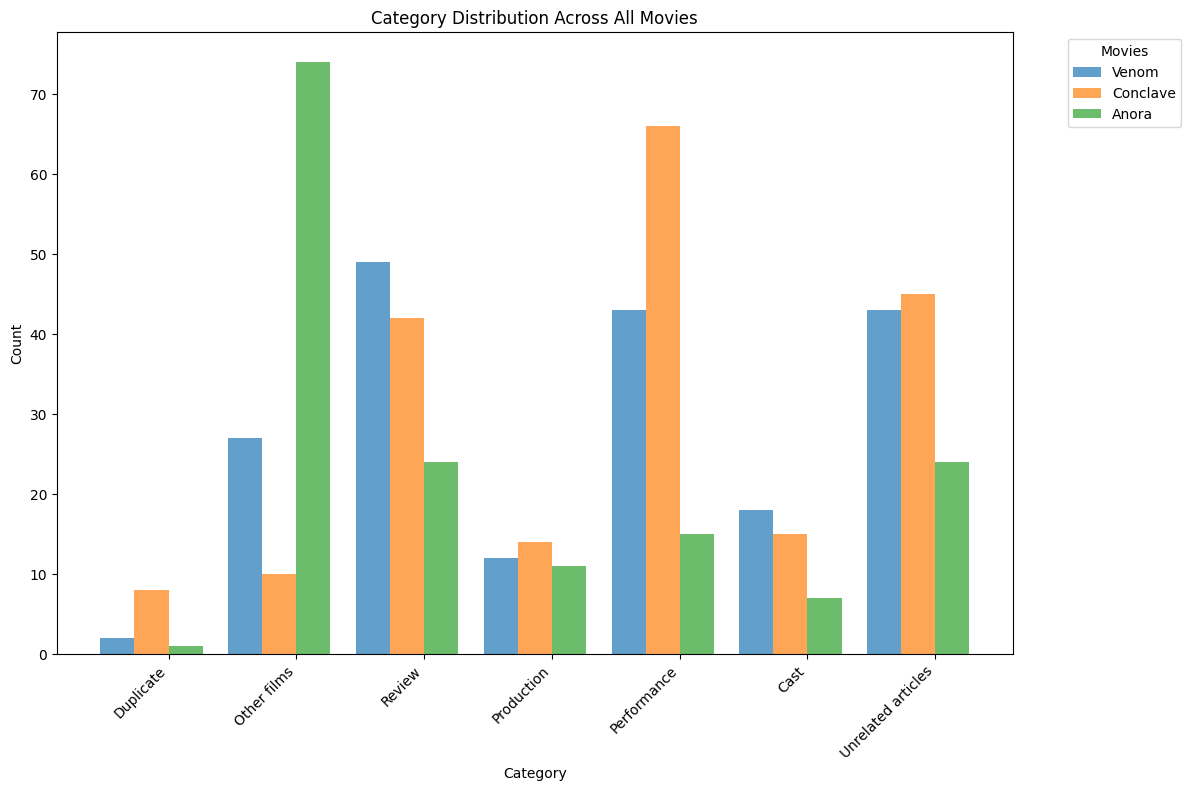
\includegraphics[width=0.9\columnwidth]{LaTeX/all_movies_distribution.png}
\caption{Distribution of Categories sorted by Movie}
\label{fig:all_movies_distribution}
\end{figure}

% Second figure
\begin{figure}[H]
\centering
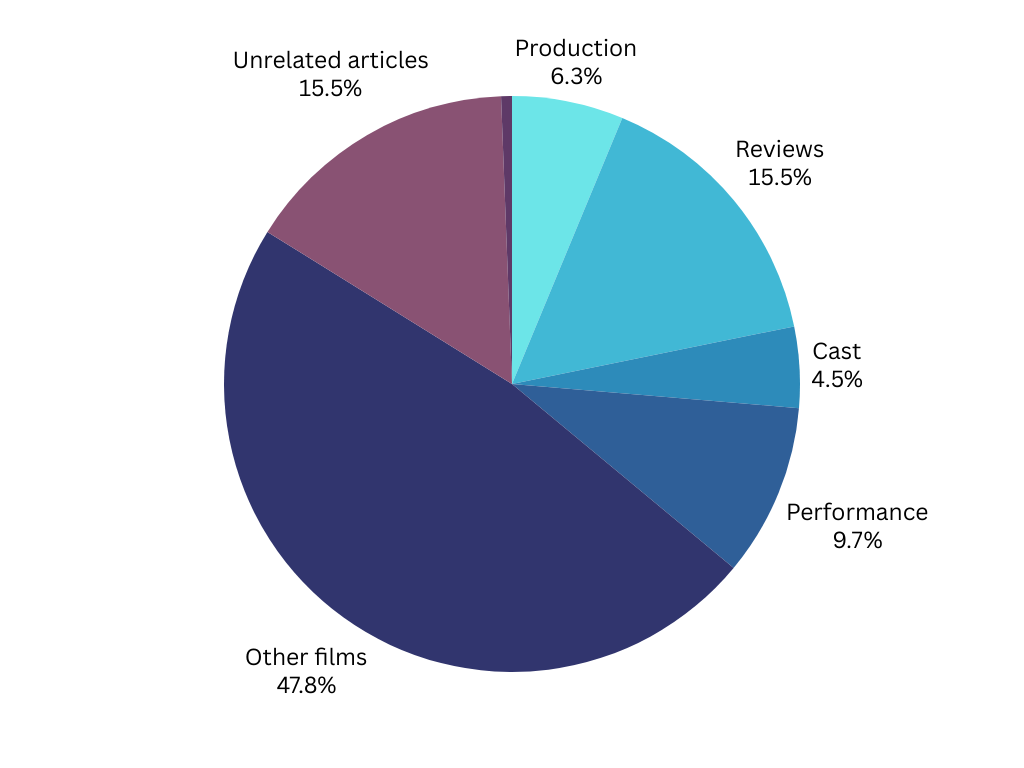
\includegraphics[width=0.9\columnwidth]{LaTeX/anora_dist.png}
\caption{Anora Distribution}
\label{fig:anora_dist}
\end{figure}

% Third figure
\begin{figure}[H]
\centering
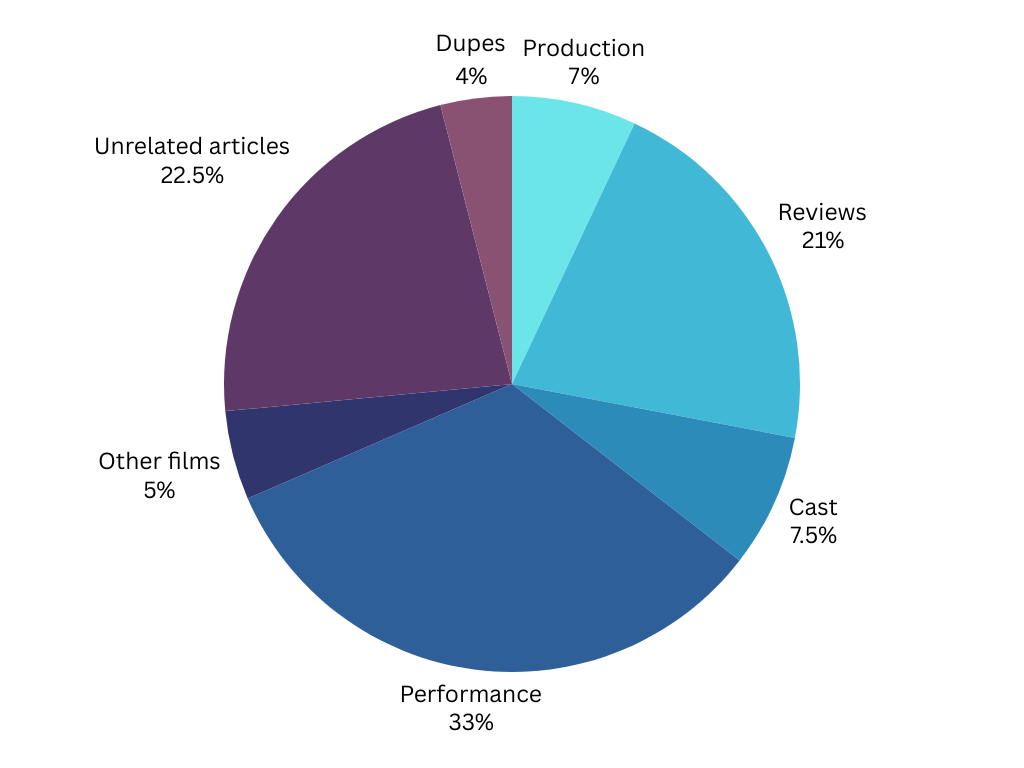
\includegraphics[width=0.9\columnwidth]{LaTeX/conclave_dist.png}
\caption{Conclave Distribution}
\label{fig:conclave_dist}
\end{figure}

% Fourth figure
\begin{figure}[H]
\centering
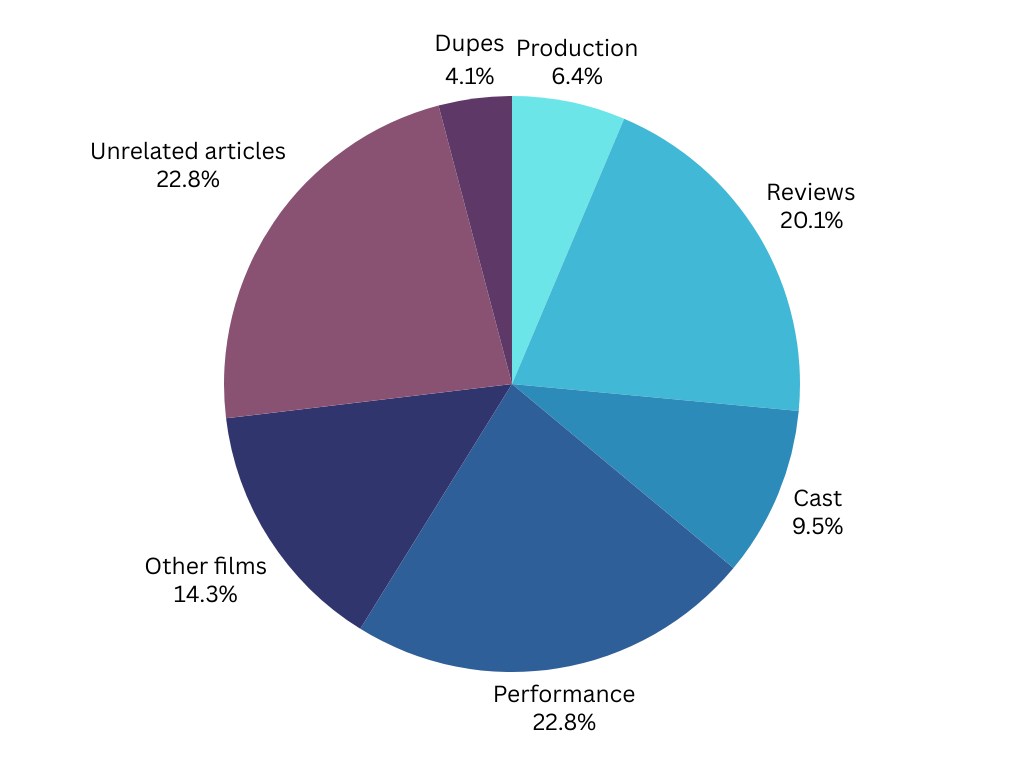
\includegraphics[width=0.9\columnwidth]{LaTeX/venom_dist.png}
\caption{Venom Distribution}
\label{fig:venom_dist}
\end{figure}

 % Ensures figures remain within this section

There are 38 articles under the “Review” category for Venom 3 and 73 articles under the “Review” category for Conclave across weeks 1 and 2, making it the most prominent category for both movies. Anora, on the other hand, only received 24 articles for the review category across both weeks. This is an indication that Venom and Conclave received more attention from critics following the 2 weeks after the release date, possibly a reflection of better visibility and coverage.

Additionally, the category “Other films” is the most dominant category for Anora in both week 1 and week 2, which contains 74 articles. There are only 10 articles for Conclave and 27 articles for Venom under the “Other films” category. A larger percentage of noise in Anora’s data is another indication that it has received less interest from media than Conclave and Venom.
While 100 articles were collected for Anora in the first week, only 60 relevant articles could be obtained from NewsAPI.org for Anora in the second week. In contrast, 100 relevant articles were obtained for Conclave and 96 relevant articles were obtained for Venom 3 in week 2, suggesting that the coverage for Anora dropped one week after its release while the other two movies had better coverage in comparison.

\subsection{Topic Characterization}
We used the TF-IDF algorithm to produce two versions of the results - one including movie names and one without movie names:
\begin{figure}[H]
\centering
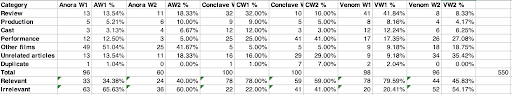
\includegraphics[width=0.9\columnwidth]{LaTeX/figure5.png}
\caption{TF-IDF Results}
\label{fig:tf-idf}
\end{figure}
Since “Review” is the top category for Venom and Conclave containing the most relevant information, we will be looking at the results for this category to compare the two different TF-IDF approaches:
\begin{figure}[H]
\centering
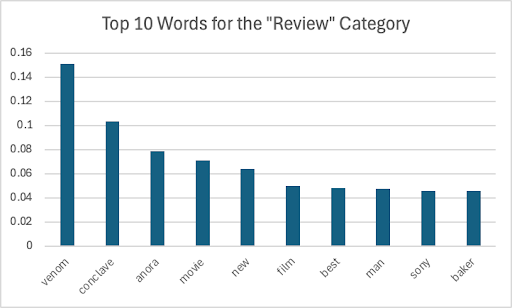
\includegraphics[width=0.9\columnwidth]{LaTeX/figure6.png}
\caption{TF-IDF Visualization of "Review" with Movie Names}
\label{fig:}
\end{figure}
\begin{figure}[H]
\centering
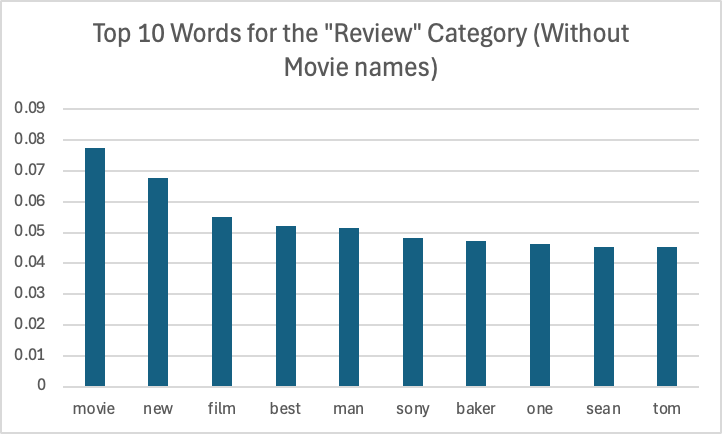
\includegraphics[width=0.9\columnwidth]{LaTeX/figure7.png}
\caption{TF-IDF Visualization of "Review" without Movie Names}
\label{fig:}
\end{figure}
It is evident that the movie names are the words with the highest TF-IDF scores for the “Review” category, suggesting that movie names are frequently mentioned when critics are reviewing the films. Since movie names are highly implied and do not provide much information for the actual category, including them can overshadow other informative words that frequently appear. It is therefore better to use the approach excluding the movie names to calculate the TF-IDF scores, which is visualized in Figure 8:

\begin{figure}[H]
\centering
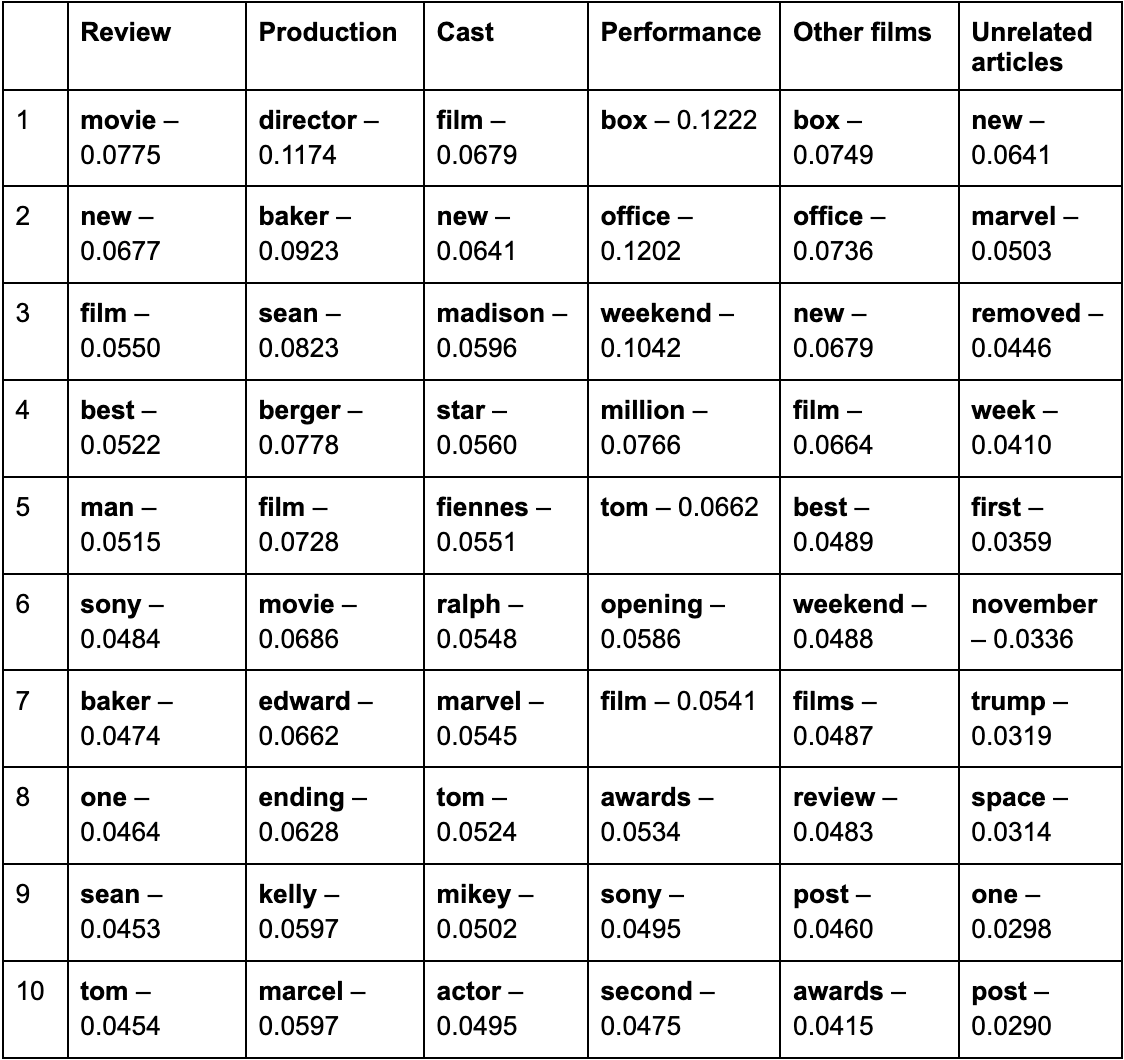
\includegraphics[width=0.9\columnwidth]{LaTeX/figure8.png}
\caption{Top 10 Words for each Category (excluding movie names)}
\label{fig:}
\end{figure}

\section {Discussion} 
\subsection{Annotated Results}
Out of the three movies, Anora had the least amount of relevant articles both relatively and absolutely, with relevant articles comprising the review, production, cast, and performance categories. In the first week of release, Anora yielded 33 relevant articles out of 96 total articles compared with 78 out of 100 for Conclave and 78 out of 98 for Venom. However, this can be attributed to differences in size or scale of the movie, both reputation and funding-wise. Conclave and Venom had budgets of \$20 million and \$120 million respectively while Anora had a budget of \$6 million. This means a difference in the amount of money allocated towards advertisement and reach. In fact, film marketers often pay or give publications and members of the press gratuitous viewing privileges in exchange for media attention. This could explain the quantitative difference in relevant articles.

Nonetheless, differences in budget are not entirely enough to justify the differences in quantity of coverage. While a budget of \$20 million is certainly more than \$6 million, it is still far less than \$120 million. Conclave is also considered an independent film and was even released by the same independent production company as Anora. Though both independent movies, Conclave might have received more media coverage than Anora because of subject matter. Conclave is a thriller about the election of a new Catholic pope and though purportedly riddled with scandal, this subject is still more respectable and appealing to a mainstream audience than the sex work spotlighted in Anora. This was still unexpected, especially considering earlier this year Anora had won the Palme d’Or, the highest prize at the prestigious Cannes Film Festival.

Between the first and second weeks after the movie’s release, Anora experienced a slight increase in the relative number of relevant articles (34.4\% to 40\%; Figure 8, referred to from here on) and a slight decrease in the number of irrelevant articles (65.6\% to 60\%). Specifically, the relative amount of reviews, production, and cast-related articles increased while performance decreased. This could be attributed to the fact that Anora was only available for limited release on October 25, 2024 and expanded to wider release on November 8, affecting the ability–especially of those who do not work for big publications and get special viewing privileges–to access, view, and comment on the movie. In fact, of all three movies, Anora had the most reviews posted by independent blogs and individuals rather than official publications. Coming from sources that have no commercial incentive, these reviews indicate more genuine critical interest and could also explain why its reviews more often involve social commentary. Conclave’s reviews also tended to entail social commentary, perhaps because both movies are about niche but real-world life situations, exploring the underbellies of sex work and religious misconduct. On the other hand, Venom is part of the Marvel franchise and far from independent, known for bringing in massive profits and crowds though not necessarily artistry. While Venom produced the greatest quantity of reviews (41 reviews vs. 13 for Anora and 32 for Conclave) in the first week post-release, these reviews were usually speculations and fan theories about cross-franchise plot/character developments rather than commentary on movie quality or greater social impact.

Conversely, both Conclave and Venom experienced large drops in the percentage of relevant articles categorized as reviews, production, or cast-related but an increase in that of performance (25\% to 41\% for Conclave, 17\% to 27\% for Venom) between the two weeks after release. The majority of these performance articles were comparing box office performance between the two weekends whereas the performance articles related to Anora were often about award nominations. This indicates that Anora was regarded with a certain prestige while Conclave and Venom were advertised more as commercial rather than independent or artistic endeavours, even though Conclave is an independent film as well. However, Conclave does happen to star two rather famous, established actors, Ralph Fiennes and Stanley Tucci, that might attract a bigger crowd whereas Anora stars mostly newcomers and foreign actors. Furthermore, the massive differences in budget mentioned earlier are definitely at play. Where more money is spent, more attention to money made is sure to follow. These observations could also be an indication that critical interest in Conclave and Venom beyond commercial performance waned in the long-term, while for Anora, critical interest persisted past the first week. 
\subsection{TF-IDF Results}

After calculating the TF-IDF scores for all the categories in our typology and excluding certain words deemed unhelpful or irrelevant to analysis, the categories of review, production, and cast yielded the most compelling results related to the reception of Anora.

\textbf{Review:} The word “best” ranks fourth in articles that are reviews and is the only qualitative word besides “new” in that category, perhaps indicating that many of the reviews involve some form of praise. It could also be part of the phrase “Best Director” or “Best Screenplay” as in the award nomination phrasing, suggesting that reviews are often written about movies that are recognized by reputable award-granting bodies as some measure of legitimacy and worth.

\textbf{Production:} “Director,” “sean,” and “baker,” are the three highest ranking words for the category of production, indicating that the director of Anora, Sean Baker, is the source of the most intrigue amongst all the crew members of all three movies. Perhaps his opinions, methods, or stylistic choices are often sought out due to his being perceived as transgressive or idiosyncratic. Edward Berger, director of Conclave, and Marcel Kelly, director of Venom, rank after Sean Baker and suggest a corresponding level of interest in these directors' talents or reputability. 

\textbf{Cast:} The names of the main leads follow a similar order with Mikey Madison of Anora appearing first followed by Ralph Fiennes of Conclave and Tom Hardy of Venom. This again points to which actors and which movies are the source of the most intrigue across all three movies and casts. Mikey Madison does play a somewhat controversial character, This is also curious considering Anora had the least overall relevant articles compared to Conclave and Venom.

\section{Group Member Contributions}
All three members took part in creating the typology, annotating the dataset, reviewing each other’s work, and creating data visualizations such as graphs, charts, and tables. Daniel produced all the code for data collection, annotation, TF-IDF calculation, and formatted the final analysis in LaTeX. Renee wrote the Introduction, Data, and Discussion sections of the report. Grace wrote the Methods and Results sections of the report.


\end{document}
